% Standalone TikZ diagram: run make in this directory for PDF and SVG.
\documentclass[11pt,tikz,border=2pt]{standalone}
% Shared typography and graph grammar for the L5a standalone TikZ diagrams.
\usepackage{fontspec}
\IfFontExistsTF{Helvetica Neue Light}{
  \setsansfont{Helvetica Neue Light}[BoldFont={Helvetica Neue Medium}]
}{\setsansfont{TeX Gyre Heros}}
\renewcommand{\familydefault}{\sfdefault}
\usepackage{amsmath,amssymb}
\usepackage{unicode-math}
\setmathfont{latinmodern-math.otf}
\usetikzlibrary{arrows.meta,calc,positioning}
\definecolor{vnslideink}{HTML}{333333}
\definecolor{vnslidebody}{HTML}{5E5E5E}
\definecolor{vnaccent}{HTML}{FF644E}
\definecolor{vnslidelink}{HTML}{579ACA}
\definecolor{vnquiet}{HTML}{899198}
\pagecolor{white}
\tikzset{
  every picture/.style={font=\sffamily\small,text=vnslidebody},
  vertex/.style={circle,draw=vnslideink,fill=white,line width=0.7pt,
    minimum size=6.4mm,inner sep=0pt,font=\sffamily\normalsize},
  edge/.style={draw=vnslidebody,line width=0.8pt,
    -{Latex[length=2.2mm,width=1.5mm]},shorten <=3.4mm,shorten >=3.4mm},
  active/.style={edge,draw=vnaccent,line width=1.2pt},
  residual/.style={edge,draw=vnslidelink,line width=1.2pt},
  inactive/.style={edge,draw=vnquiet,line width=0.7pt},
  edge label/.style={fill=white,inner sep=1.4pt,font=\sffamily\small},
  partition/.style={rounded corners=2mm,line width=0.5pt},
}

\begin{document}
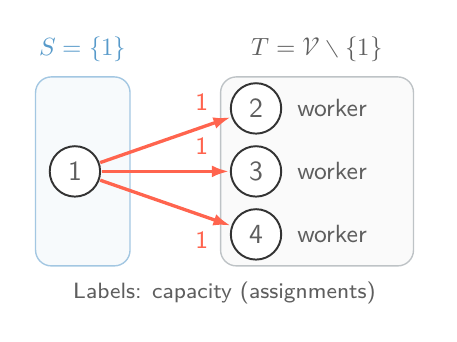
\begin{tikzpicture}[x=1cm,y=1cm]
  % Only the three actual source-to-worker edges are drawn.
  % T also contains all task, completion, and sink vertices.
  \draw[partition,draw=vnslidelink!55,fill=vnslidelink!5]
    (-0.5,-1.2) rectangle (0.7,1.2);
  \draw[partition,draw=vnquiet!55,fill=black!2]
    (1.85,-1.2) rectangle (4.3,1.2);
  \coordinate (s) at (0,0);
  \coordinate (w2) at (2.3,0.8);
  \coordinate (w3) at (2.3,0);
  \coordinate (w4) at (2.3,-0.8);
  \draw[active] (s)--node[edge label,pos=0.7,above=4pt,text=vnaccent]{1}(w2);
  \draw[active] (s)--node[edge label,pos=0.7,above=4pt,text=vnaccent]{1}(w3);
  \draw[active] (s)--node[edge label,pos=0.7,below=4pt,text=vnaccent]{1}(w4);
  \node[vertex] at (s) {1};
  \foreach \i in {2,3,4} {
    \node[vertex] at (w\i) {\i};
    \node[right=4mm,font=\sffamily\small] at (w\i) {worker};
  }
  \node[text=vnslidelink] at (0.1,1.55) {$S=\{1\}$};
  \node at (3.075,1.55) {$T=\mathcal V\setminus\{1\}$};
  \node[font=\sffamily\footnotesize] at (1.9,-1.55) {Labels: capacity (assignments)};
  \path[use as bounding box] (-0.6,-1.8) rectangle (4.5,1.8);
\end{tikzpicture}
\end{document}
